\documentclass[11pt]{article}

\usepackage[headings]{fullpage}
\usepackage[utopia]{mathdesign}
\usepackage{color}
\usepackage{graphicx}

\pagestyle{myheadings}
\markboth{Magic}{Magic}

\usepackage{amsmath}
\usepackage{bm}
\usepackage[T1]{fontenc}
\usepackage{matlab-prettifier}

\newcommand{\nat}{\mathbb{N}}          % Natural numbers
\newcommand{\integer}{\mathbb{Z}}      % Integers
\newcommand{\real}{ {\mathbb{R}} }     % Reals
\newcommand{\float}{ {\mathbb{F}} }     % Reals
\newcommand{\rmn}[2]{ \mathbb{R}^{#1\times#2} }     % Reals
\newcommand{\complex}{ {\mathbb{C}} }  % Complex
\newcommand{\macheps}{\ensuremath \varepsilon_{\text{mach}}}

\renewcommand{\Re}{\operatorname{Re}}
\renewcommand{\Im}{\operatorname{Im}}

% Boldface vectors
\newcommand{\bff}{\bm{f}}
\newcommand{\bfF}{\bm{F}}
\newcommand{\bfw}{\bm{w}}
\newcommand{\bfv}{\bm{v}}
\newcommand{\bfe}{\bm{e}}
\newcommand{\bfc}{\bm{c}}
\newcommand{\bfp}{\bm{p}}
\newcommand{\bfq}{\bm{q}}
\newcommand{\bfr}{\bm{r}}
\newcommand{\bfs}{\bm{s}}
\newcommand{\bfu}{\bm{u}}
\newcommand{\bfb}{\bm{b}}
\newcommand{\bfx}{\bm{x}}
\newcommand{\bfy}{\bm{y}}
\newcommand{\bfg}{\bm{g}}
\newcommand{\bfh}{\bm{h}}
\newcommand{\bfz}{\bm{z}}
\newcommand{\bfa}{\bm{a}}
\newcommand{\bft}{\bm{t}}
\newcommand{\bfd}{\bm{d}}
\newcommand{\bfalpha}{\bm{\alpha}}
\newcommand{\bfeps}{\bm{\varepsilon}}
\newcommand{\bfdelta}{\bm{\delta}}
\newcommand{\bfzero}{\bm{0}}
\newcommand{\eye}[1]{\bfe_{#1}}

% Boldface matrix
\newcommand{\m}[1]{\bm{#1}}
\newcommand{\mA}{\m{A}}
\newcommand{\mL}{\m{L}}
\newcommand{\mF}{\m{F}}
\newcommand{\mU}{\m{U}}
\newcommand{\mJ}{\m{J}}
\newcommand{\mP}{\m{P}}
\newcommand{\mQ}{\m{Q}}
\newcommand{\mR}{\m{R}}
\newcommand{\mD}{\m{D}}
\newcommand{\mS}{\m{S}}
\newcommand{\mB}{\m{B}}
\newcommand{\mC}{\m{C}}
\newcommand{\mE}{\m{E}}
\newcommand{\mG}{\m{G}}
\newcommand{\mH}{\m{H}}
\newcommand{\mV}{\m{V}}
\newcommand{\mW}{\m{W}}
\newcommand{\mX}{\m{X}}
\newcommand{\mZ}{\m{Z}}
\newcommand{\mK}{\m{K}}
\newcommand{\mM}{\m{M}}

\newcommand{\meye}{\m{I}}

\newcommand{\ee}[1]{\times 10^{#1}}
\newcommand{\jac}[2]{\frac{\bfd \bm{#1}}{\bfd \bm{#2}}}
\newcommand{\diag}{\operatorname{diag}}
\newcommand{\fl}{\operatorname{fl}}
\newcommand{\circop}[1]{\makebox[0pt][l]{$\bigcirc$}\hspace{1pt}#1}
\newcommand{\myvec}{\operatorname{vec}}
\newcommand{\unvec}{\operatorname{unvec}}
\newcommand{\kron}[2]{#1 \otimes #2}

% matlab stuff
\lstset{style=Matlab-editor,basicstyle=\mlttfamily}
\newcommand{\Mfile}[1]{\lstinputlisting[]{#1}}
\lstnewenvironment{matlab}%
  {\lstset{escapechar=`}}%
  {}
\lstMakeShortInline[style=Matlab-editor,basicstyle=\mlttfamily]"  % use " for inline code
\newcommand{\matlabend}{\lstinline[style=Matlab-style,basicstyle=\mlttfamily,mloverride=true]!end!}


\begin{document}

\begin{center}
  \bf Do you believe in magic?
\end{center}

Magic squares have fascinated humanity for centuries. In our
terminology, a magic square is an $n\times n$ matrix whose entries are
the integers from 1 to $n^2$, arranged so that the sum of every row,
every column, and the two long diagonals is the magic number
$n(n^2+1)/2$. 

A famous example is Durer's magic square,
\[
\begin{bmatrix}
  16 & 3 & 2 & 13 \\ 5 & 10 & 11 & 8 \\ 9 & 6 & 7 & 12 \\ 4 & 15 & 14 & 1
\end{bmatrix}
\]
One of the coolest facts about this magic square is that it contains the numbers 15 and 14 next to each other, and in 1514 he made an engraving about it:
\begin{center}
  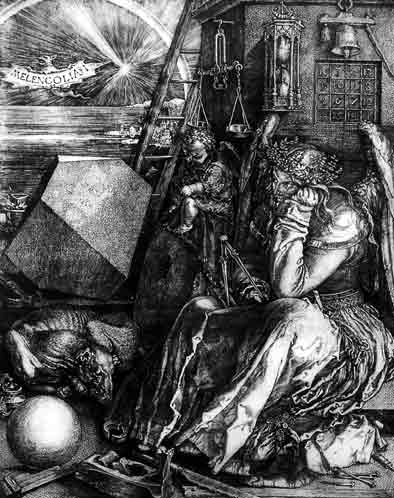
\includegraphics[height=2in]{durer}
\end{center}
It has a couple more tricks up its sleeve as well.

We can check the magic square properties with a little linear algebra. First consider the inner product 
\begin{equation}
	\label{ones}
\begin{bmatrix}
a & b & c & d 
\end{bmatrix} \begin{bmatrix}
1 \\ 1 \\ 1 \\ 1
\end{bmatrix}
= a + b + c + d,
\end{equation}
allowing us to sum the entries of a vector. We can do something similar with the square matrix $M$, summing all the rows simultaneously:
\begin{equation}
	\label{Mones}
	M \begin{bmatrix}
		1 \\ 1 \\ 1 \\ 1
	\end{bmatrix}
	= 1 \bm{m}_1 + 1 \bm{m}_2 + 1 \bm{m}_3 + 1 \bm{m}_4.
\end{equation}
The result is a column vector, each entry of which is the sum of elements in its row. To sum columns instead, we can first transpose $M$ so that the columns become rows. Finally, note that if $\mA$ is $n\times n$ and $\bfx$ is a column vector of $n$ ones, then we can do two multiplications and get
\begin{equation}
	\label{sumall}
	\bfx^T \mA \bfx = \bfx^T ( \bfa_1 + \cdots + \bfa_n) = \sum_{i=1}^n \sum_{j=1}^n A_{ij}.
\end{equation}


\subsection*{Preparation}

Read section 2.2, and the online help for the \texttt{diag} command.

\subsection*{Goals}

You will use MATLAB commands to manipulate Durer's magic square and check its special properties. While you could do all the operations by summing in loops, we'll use linear algebra techniques that make vectors and matrices the central focus.

\subsection*{Required submission elements}

Download the template script and complete it to do the following. You should use the techniques described in the introduction. 

\begin{enumerate}
\item Let \texttt{M} be Durer's magic square as given above. 
\item Use the matrix-vector multiplication in~\eqref{Mones} to compute the row sums of $M$.  
\item Use a transpose and~\eqref{Mones} to compute the column sums of $M$. 
\item There are four $2\times 2$ submatrices made by drawing lines
  horizontally and vertically through the center of the matrix. Using the identity~\eqref{sumall}, verify that the sum of the elements of each of these submatrices is also the magic number.
\item There is another $2\times 2$ submatrix made by the four interior elements. Verify that the sum of these elements is---wait for it---the magic number. 
\item Find the sum of the main diagonal of \texttt{M} using \texttt{diag} and~\eqref{ones}. Then do the same for the sum on the ``antidiagonal.'' (Hint: How can you rearrange $M$ so that the antidiagonal becomes the diagonal?)
\end{enumerate}


\end{document}

%%% Local Variables:
%%% mode: latex
%%% TeX-master: t
%%% End:
